\documentclass[10pt]{article} % Font size - 10pt, 11pt or 12pt

\usepackage{amsmath}
\usepackage[hmargin=1.25cm, vmargin=1.5cm]{geometry} % Document margins

\usepackage[usenames,dvipsnames]{xcolor} % Allows the definition of hex colors

% Fonts and tweaks for XeLaTeX
\usepackage{fontspec,xltxtra,xunicode}
\defaultfontfeatures{Mapping=tex-text}
%\setmonofont[Scale=MatchLowercase]{Andale Mono}

% Colors for links, text and headings
\usepackage{hyperref}
\definecolor{linkcolor}{HTML}{506266} % Blue-gray color for links
\definecolor{shade}{HTML}{F5DD9D} % Peach color for the contact information box
\definecolor{text1}{HTML}{2b2b2b} % Main document font color, off-black
\definecolor{headings}{HTML}{701112} % Dark red color for headings
% Other color palettes: shade=B9D7D9 and linkcolor=A40000; shade=D4D7FE and linkcolor=FF0080

\hypersetup{colorlinks,breaklinks, urlcolor=linkcolor, linkcolor=linkcolor} % Set up links and colors

\usepackage{fancyhdr}
\pagestyle{fancy}
\fancyhf{}
% Headers and footers can be added with the \lhead{} \rhead{} \lfoot{} \rfoot{} commands
% Example footer:
%\rfoot{\color{headings} {\sffamily Last update: \today}. Typeset with Xe\LaTeX}

\renewcommand{\headrulewidth}{0pt} % Get rid of the default rule in the header
\renewcommand{\baselinestretch}{1.2}

\usepackage{titlesec} % Allows creating custom \section's

% Format of the section titles
\titleformat{\section}{\color{headings}
\scshape\Large\raggedright}{}{0em}{}[\color{black}\titlerule]

\title{Using the Phase-Field model for Creating Anisotropic Crystals}
\author{Elliott Capek}

\begin{document}
\maketitle{}

\section{Introduction}
The Phase-Field model is a method for simulating phase transitions in systems. Phase transitions in real life are discontinuous, making them hard to represent analytically. The Phase-Field method overcomes this by representing the phase of a region with a space- and time-dependent function $\phi(r,t)$. $\phi$ ranges from $0$ to $1$, with either end of the range being one phase or the other, and numbers between $0$ and $1$ representing transitional regions. These transitional regions, while not physical, can approximate reality well if the distance between a 0-zone and a 1-zone is as small as possible. \\

In this paper we seek to reproduce the results of Sanal [1], where a solid-liquid phase transition with anisotropic dependence is time-evolved. The anisotropy (angular dependence) of the equations used in this paper allow for radially-symmetric crystals to form. In this formulation, $\phi=1$ corresponds to solid phase and $\phi=0$ corresponds to liquid phase. The equation for time-evolving $\phi$ is given in Sanal as:

\begin{equation}  \label{eq:dPhidt}
  \tau \frac{\partial \phi}{\partial t} = -\frac{\partial}{\partial x} \left(\epsilon \frac{d\epsilon}{d\theta}\frac{\partial\phi}{\partial y}\right) + \frac{\partial}{\partial y} \left(\epsilon \frac{d\epsilon}{d\theta}\frac{\partial \phi}{\partial x}\right) + \nabla \cdot \left(\epsilon^2\nabla\phi\right) + \phi\left(1-\phi\right)\left(\phi-0.5+m\right)
\end{equation}

Here $\tau$ is the relaxation time, or the time it takes $\phi$ to come into equilibrium with its neighbors. $\epsilon$ is a small $\theta$-dependent parameter which controls how quickly the solid-liquid interface moves. $\theta$ is the angle from the origin measured from the horizontal. Making $\epsilon$ depend on $\theta$ introduces anisotropy into the model, allowing different angles to spread at different rates. $m$ is the thermodynamic driving force, a temperature-dependent number which determines how favorable solidification is. Larger values of temperature (and hence $m$) correspond to quicker solidification. \\

\section{Derivation of $\phi$-evolution}
The derivation of the equation for $\frac{d\phi}{dt}$ begins with a free energy functional:

\begin{equation}
  F = \int f(\phi,m) + \frac{\epsilon(\phi)^2}{2}|\nabla\phi|^2 dV
\end{equation}

F, the free energy, is a functional of $\phi(r,t)$ and $\epsilon(\phi)$. The above equation has two components: function $f(\phi,m)$, which is the potential energy of the system, and the $\epsilon$ term, which represents the surface tension of the crystal.\\

Potential f only needs to be defined between $\phi=0$ and $\phi=1$, due to the definition of $\phi$. f should have local minima at $\phi=0$ and $\phi=1$ to encourage settling at either phase and discourage transitional values of $\phi$. The potential is also m-dependent. m is the thermodynamic driving force of the phase-change reaction. It decides if it is favorable or unfavorable to be a solid or liquid, and is a function of T. Potential depends on m in that the higher m is, the more favorable the liquid phase should be. Sanal presents the following as the phase-transition potential:

\begin{equation}
  f(\phi,m) = \frac{1}{4}\phi^4 - \left(\frac{1}{2} - \frac{1}{3}m\right)\phi^3 + \left(\frac{1}{4}-\frac{1}{2}m\right)\phi^2
\end{equation}

This polynomial meets all the above requirements. See Figure (\ref{fig:f}) for a plot of potential.\\

Thermodynamic driving force m is given by the following equation:

\begin{equation}
  m = \frac{\alpha \tan^{-1}\left(\gamma\left(T_{eq}-T\right)\right)}{\pi}
\end{equation}

where $\alpha \leq 1$ and $\gamma$ are positive constants. By this definition, $|m| \leq \frac{1}{2}$.

\begin{figure}[h!]
  \caption{\textbf{A plot of $f(\phi,m)$ for different values of m. Notice that all lines have minima at $\phi=0$ and $\phi=1$. The general trend is higher values of m have higher potentials for the solid phase. At m=0, there is an equal potential for solid and liquid phase, hence this is the equilibrium m (corresponding to an equilibrium temperature).}}
  \centering
  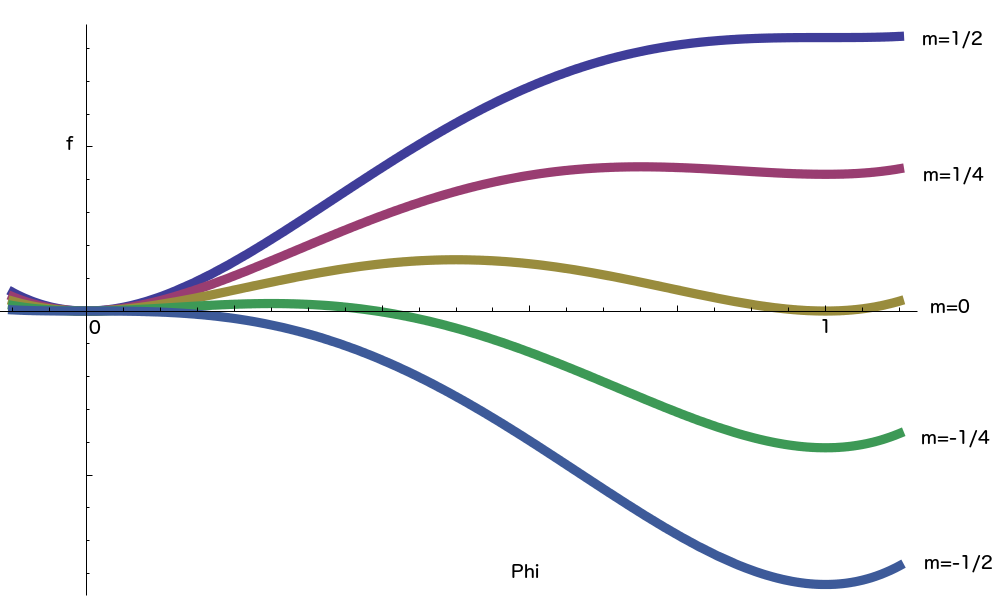
\includegraphics[width=0.5\textwidth]{../f_plot.png}
  \label{fig:f}
\end{figure}

The epsilon term in the F functional exists to make the phase-transition region as small as possible, and also to introduce anisotropy. The potential f discourages $\phi$ from taking transition values, but it isn't detailed enough. It discourages transition values system-wide, but we want to make the transition region as small as possible. This requires a $\nabla\phi$, which is present in the $\epsilon$-term. The larger $\nabla\phi$, the smaller the solid-liquid interface will be. Because we want to encourage small solid-liquid as well as liquid-solid transitions, the gradient term becomes $|\nabla\phi|$. The actual $\epsilon(\phi)$ function controls where $\phi$ should change. This $\epsilon$ is actually a function of the negative gradient of phi, $\epsilon(-\nabla\phi)$ since it only depends on the angle of the interface. This is to introduce anisotropy. $\epsilon$ is defined as follows:

\begin{equation}
  \epsilon = 1 + \delta\cos(j(\phi_0-\phi))
\end{equation}

where $\delta$ is a small value which controls strength of anisotropy, $j$ controls how many angular nodes show up, and $\phi_0$ rotates the crystal. The basic function of $\epsilon$ is to control where the phase-transition should appear, or in this case, how expensive certain angles of the phase transition should be. Certain angles are cheap, and so the system will have the barrier take those on, and some will be expensive, so the system will try and minimize the area of the interface at that angle. In particular, values of $j(\phi_0-\phi)$ close to $-1$ will be favored and values close to $1$ will be disfavored.\\

The free energy functional is a value that is minimized when a system evolves in time. We can use this fact to time-evolve $\phi$. Intuitively we know that, if we want to minimize F by changing $\phi$, we should couple $\frac{\partial\phi}{\partial t}$ to the functional derivative $\frac{\delta F}{\delta \phi}$, or how much free energy is changing with respect to a change in $\phi$. Sanal does this as follows:

\begin{equation}
  \tau \frac{\partial \phi}{\partial t} = \frac{\delta F}{\delta \phi}
\end{equation}

where $\tau$ is a small positive parameter which controls the proportionality of the two derivatives. This functional derivative is difficult to evaluate. We can transform this equation into a simpler numerical one like so:

\begin{equation}
  \tau \frac{d\phi_{ij}}{dt} = \frac{dF_{ij}}{d\phi_{ij}}
  \label{eq:phi-evol}
\end{equation}

Becuse we are on a two-dimensional grid, we can compartmentalize $\phi$, so $\phi_{ij}$ is the $(i,j)$ element on our grid. Free energy F is an integral over the entire system, but we can compartmentalize it to the following:

\begin{equation}
  F_{ij}(\phi_{ij}) = f(\phi_{ij},m) + \frac{\epsilon(\phi_{ij})^2}{2}|\nabla\phi_{ij}|^2
\end{equation}

where we have removed the volume integral on the total F. We can see that $F = \sum_i \sum_j F_{ij}$, so minimizing F is equivalent to minimizing $F_{ij}$ for all values of $i,j$. We have transformed the functional F into a simple function $F_{ij}$.\\

NOTE: One problem with Equation (\ref{eq:phi-evol}) to me is that $\tau$ should be negative. It seems that if $\frac{dF_{ij}}{d\phi_{ij}}$ is positive, then $\frac{d\phi_{ij}}{dt}$ should be negative, so as to make sure $F_{ij}$ is always decreasing as time increases. However, this equation seems to predict the opposite.\\

We then take the $\phi$ derivative of the RHS of Equation (\ref{eq:phi-evol}) and get the following:

\begin{equation}
  \tau \frac{d\phi_{ij}}{dt} = \frac{\partial}{\partial x}\left(\epsilon_{ij}\frac{\partial \epsilon_{ij}}{\partial \phi_{ij}}\frac{\partial \phi_{ij}}{\partial y}\right) + \frac{\partial}{\partial y}\left(\epsilon_{ij}\frac{\partial \epsilon_{ij}}{\partial \phi}\frac{\partial \phi_{ij}}{\partial x}\right) + \epsilon_{ij}^2\nabla^2\phi_{ij} + \phi_{ij}\left(1-\phi_{ij}\right)\left(\phi_{ij}-0.5+m\right)
\end{equation}

The fourth term is a rearrangement of $-\frac{\partial f}{\partial\phi}$. The first three terms are part of the product rule derivation of $\frac{\epsilon^2}{2}|\nabla\phi|^2$. This equation is in a form that we can evaluate numerically.

\section{Derivation of T-evolution}

Temperature evolution is done with the following equation:

\begin{equation}
  \frac{\partial T}{\partial t} = \nabla^2 T + K\frac{\partial\phi}{\partial t}
\end{equation}

The first term is the normal heat equation, where heat is passed from high-temperature elements to low-temperature elements. The second term is the heat evolved from the transition from liquid to solid. K is the latent heat, which describes how much heat is released at this transition.

\section{Simulation}
Now that we have our time-evolution equations, it is a simple matter to solve for $\phi$ over time. We do this by using the forwards-Euler method on equations (11) and (12), which requires us to compute spacial derivatives of $\frac{\partial}{\partial x}\left(\epsilon_{ij}\frac{\partial \epsilon_{ij}}{\partial \phi_{ij}}\frac{\partial \phi_{ij}}{\partial y}\right)$ and $\frac{\partial}{\partial y}\left(\epsilon_{ij}\frac{\partial \epsilon_{ij}}{\partial \phi}\frac{\partial \phi_{ij}}{\partial x}\right)$, as well as the Laplacian of both $\epsilon$ and $\phi$. We compute the spacial derivatives of the functions by taking the difference between the values at neighboring points (using periodic boundary conditions). We use a nine-point Laplacian using the considered point and the eight points adjacent to it, weighting the adjacent points $+\frac{2}{3}$ and the considered point $-4$.

\section{Reference}
        \hspace{2cm}[1] Sanal, Rahul. Numerical Simulation of Dendritic crystal growth using phase field method and investigating the effects of different physical parameter on the growth of the dendrite. Arxiv.<arxiv.org/ftp/arxiv/papers/1412/1412.3197.pdf>\\

\end{document}
